% =========================================================
%  Chapter 7 — Heterostructure Materials, Carrier Dynamics,
%              and the Gain Rate Equation
%  Source: Dr. George's Lectures (Lecture 3)
%  Style: student-voice notes matching the personal style guide
% =========================================================

% ------------------------------------------------------------------
\section{Completing the Heterostructure Picture}
% ------------------------------------------------------------------

The previous chapter established the double heterostructure as the engineering solution to the homojunction's two fundamental problems — a thick, unconfined gain region and a weak optical mode overlap. We saw that the narrow-gap active layer simultaneously traps carriers via band-edge discontinuities and guides photons via its higher refractive index. One key fact was stated but not yet fully explained: \emph{why} does a smaller bandgap automatically imply a higher refractive index? And once we accept the heterostructure architecture, how do we actually choose the right material system for a given target wavelength while guaranteeing that the crystal interfaces are defect-free? This chapter answers both questions before building the complete dynamical model of how carriers and photons interact inside the device.

% ------------------------------------------------------------------
\section{Why Smaller Bandgap Means Higher Refractive Index}
% ------------------------------------------------------------------

The link between bandgap and refractive index is not a coincidence — it is a direct consequence of the Kramers-Kronig relations, the same causality constraint that links the real and imaginary parts of any complex response function. The same principle that ties the real part of the atomic susceptibility to its imaginary (absorptive) part applies here, now to the complex refractive index $\tilde{n} = n + j\kappa$ of the semiconductor.

To see how this relation is derived, we start from the principle of causality, which dictates that the polarization response of a medium at time $t$ can only depend on the electric field at prior times $t' \le t$. In the time domain, the dielectric susceptibility $\chi(t)$ must therefore vanish for $t < 0$. The Fourier transform of this causal response is:
\begin{equation*}
    \chi(\omega) = \int_0^\infty \chi(t) e^{j\omega t} dt
\end{equation*}
Because the integration is restricted to $t \ge 0$, the function $\chi(\omega)$ is analytic in the upper half of the complex frequency plane ($\text{Im}(\omega) > 0$). Applying Cauchy's integral theorem along a contour that runs along the real axis (with an infinitesimal semicircle bypassing the pole at $\omega' = \omega$) and is closed by a large semicircle at infinity yields:
\begin{equation*}
    \chi(\omega) = \frac{1}{j\pi}\,\mathcal{P}\int_{-\infty}^{\infty} \frac{\chi(\omega')}{\omega' - \omega}\,d\omega'
\end{equation*}
Splitting the susceptibility into real and imaginary parts, $\chi(\omega) = \chi'(\omega) + j\chi''(\omega)$, and equating the real parts:
\begin{equation*}
    \chi'(\omega) = \frac{1}{\pi}\,\mathcal{P}\int_{-\infty}^{\infty} \frac{\chi''(\omega')}{\omega' - \omega}\,d\omega'
\end{equation*}
Since the time-domain susceptibility $\chi(t)$ is a real quantity, the frequency-domain susceptibility must satisfy the crossing relation $\chi(-\omega) = \chi^*(\omega)$, which implies $\chi'(-\omega) = \chi'(\omega)$ and $\chi''(-\omega) = -\chi''(\omega)$. Splitting the integration domain into positive and negative frequencies and substituting $\omega' \to -\omega'$ for the negative portion, we obtain:
\begin{align*}
    \chi'(\omega) &= \frac{1}{\pi}\,\mathcal{P}\left[ \int_{0}^{\infty} \frac{\chi''(\omega')}{\omega' - \omega}\,d\omega' + \int_{0}^{\infty} \frac{-\chi''(\omega')}{-\omega' - \omega}\,d\omega' \right] \\
    &= \frac{1}{\pi}\,\mathcal{P} \int_{0}^{\infty} \chi''(\omega') \left[ \frac{1}{\omega' - \omega} + \frac{1}{\omega' + \omega} \right] d\omega' \\
    &= \frac{2}{\pi}\,\mathcal{P}\int_0^\infty \frac{\omega'\,\chi''(\omega')}{\omega'^2 - \omega^2}\,d\omega'
\end{align*}
Finally, the complex refractive index is related to the dielectric function by $\tilde{n} = n + j\kappa = \sqrt{1 + \chi}$. For a weakly polarizable medium, we can approximate $\tilde{n} - 1 \approx \chi/2$, which yields $n(\omega) - 1 \approx \chi'(\omega)/2$ and $\kappa(\omega) \approx \chi''(\omega)/2$. Substituting these approximations into the susceptibility relation directly yields the Kramers-Kronig integral for the real refractive index $n(\omega)$:
\begin{keyresult}
    \begin{equation}
        n(\omega) - 1 = \frac{2}{\pi}\,\mathcal{P}\int_0^{\infty}\frac{\omega'\,\kappa(\omega')}{\omega'^2 - \omega^2}\,d\omega'
    \end{equation}
\end{keyresult}
where $\mathcal{P}$ denotes the Cauchy principal value of the integral. Physically, this equation says that $n(\omega)$ at any given frequency is determined by the \emph{entire} absorption spectrum $\kappa(\omega')$ of the material. The key insight is in the weighting: the $1/(\omega'^2 - \omega^2)$ denominator gives the largest contributions from $\omega'$ close to $\omega$.

\begin{figure}[H]
    \centering
    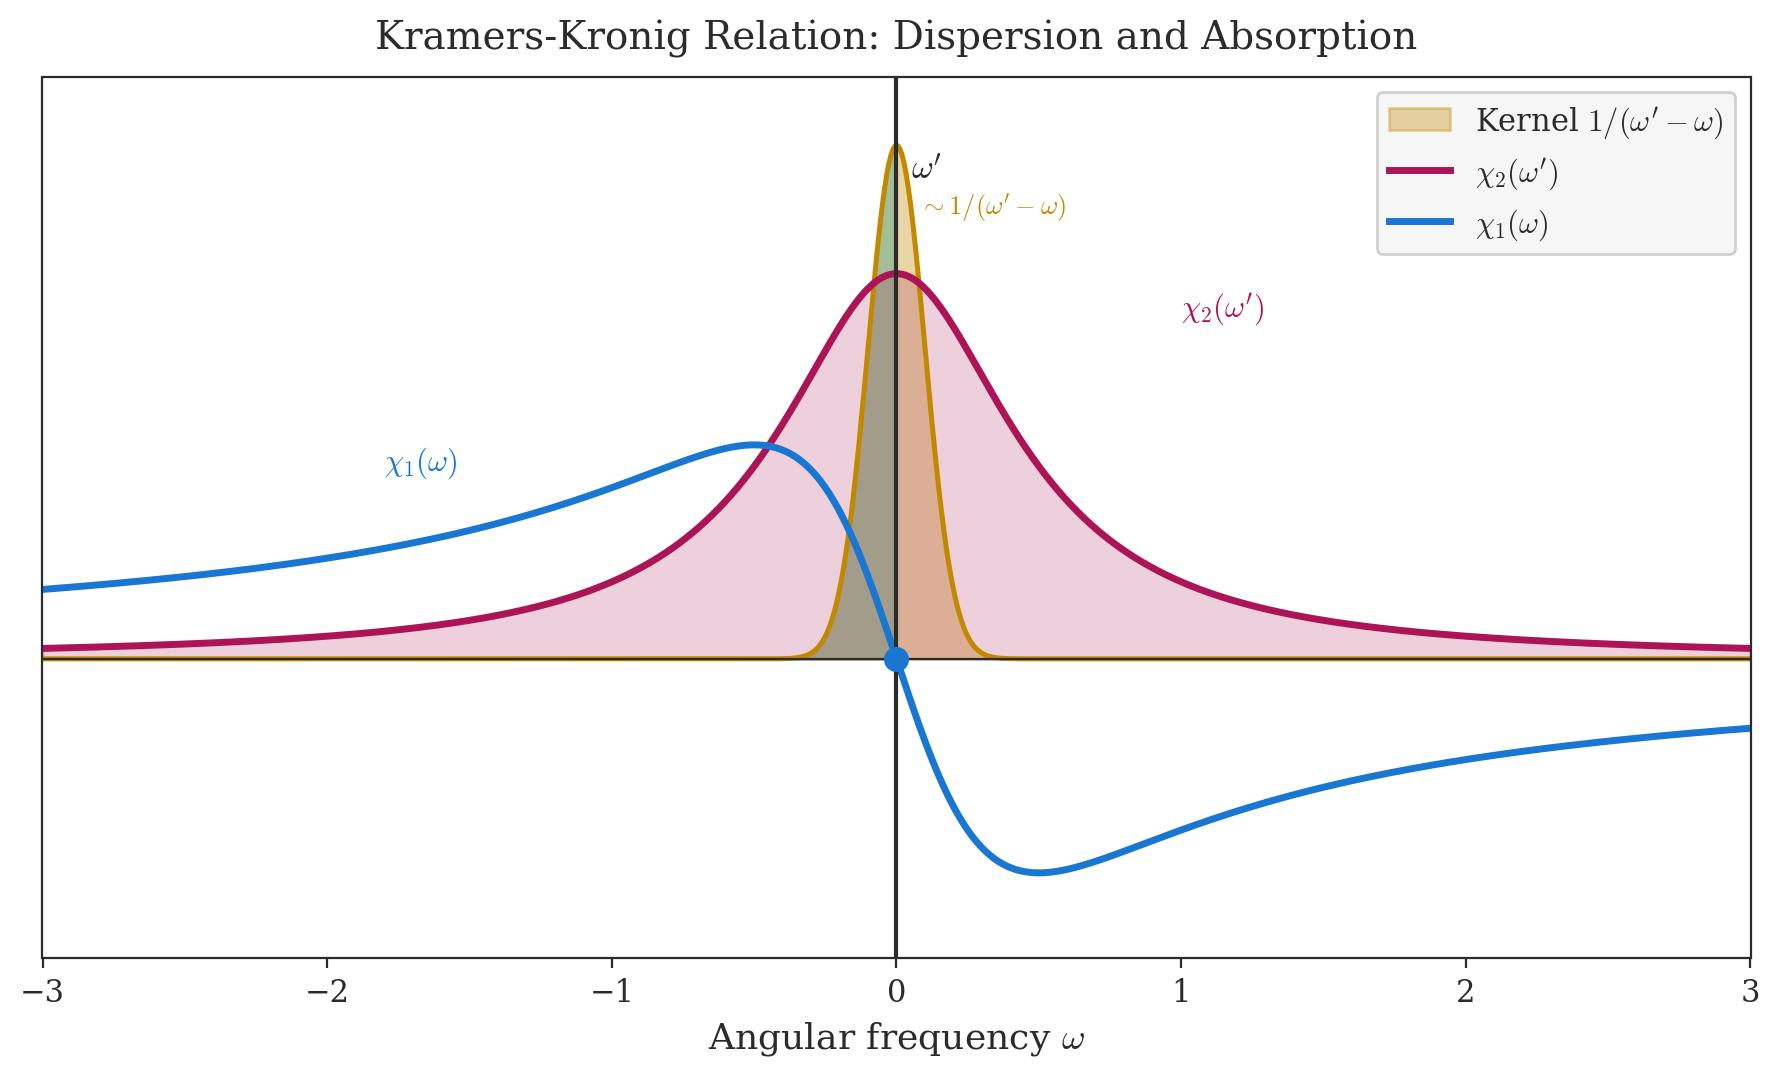
\includegraphics[width=0.6\textwidth]{Figures/Chapter 7/kramers_kronig.jpg}
    \caption{Kramers–Kronig Relation: Real and Imaginary Refractive Index}
    \label{fig:kramers_kronig}
\end{figure}

Now consider two materials: one with a small bandgap (like GaAs, $E_g \approx 1.42\,\text{eV}$) and one with a large bandgap (like AlAs, $E_g \approx 2.16\,\text{eV}$). The small-gap material begins absorbing photons at a much lower frequency — its $\kappa(\omega')$ has a nonzero contribution starting from $\omega' = E_g/\hbar$ which is comparatively small. When we integrate this contribution into the Kramers-Kronig formula, the lower-frequency onset of absorption dominates the integral at any optical operating frequency below the bandgap. The result: smaller-gap materials accumulate a larger integral, which yields a higher real refractive index $n$.

This is precisely why the active layer of a double heterostructure — which must have the smallest bandgap in the stack to enable photon emission — automatically has a higher refractive index than its wider-gap cladding layers. \textbf{The carrier confinement and photon confinement functions of the heterostructure are not independent design choices: they both flow from the single constraint that the active material must have the smallest bandgap.}

% ------------------------------------------------------------------
\section{Materials Design for Heterojunctions}
% ------------------------------------------------------------------

\subsection{Binary Semiconductors: The Starting Point}

The simplest III-V semiconductors are binary compounds — one Group-III element paired with one Group-V element. The most important property determining suitability for light emission is whether the bandgap is direct or indirect. Group-IV elemental semiconductors (Si, Ge) have indirect bandgaps: their conduction band minimum sits at a different crystal momentum than the valence band maximum, so any optical transition requires a phonon to supply the momentum difference, making radiative recombination a three-particle process that is enormously less probable. The III-V binaries frequently have direct gaps — conduction minimum and valence maximum at the same $k$-point — making them the foundation of all practical LED and laser technology.

\begin{figure}[H]
    \centering
    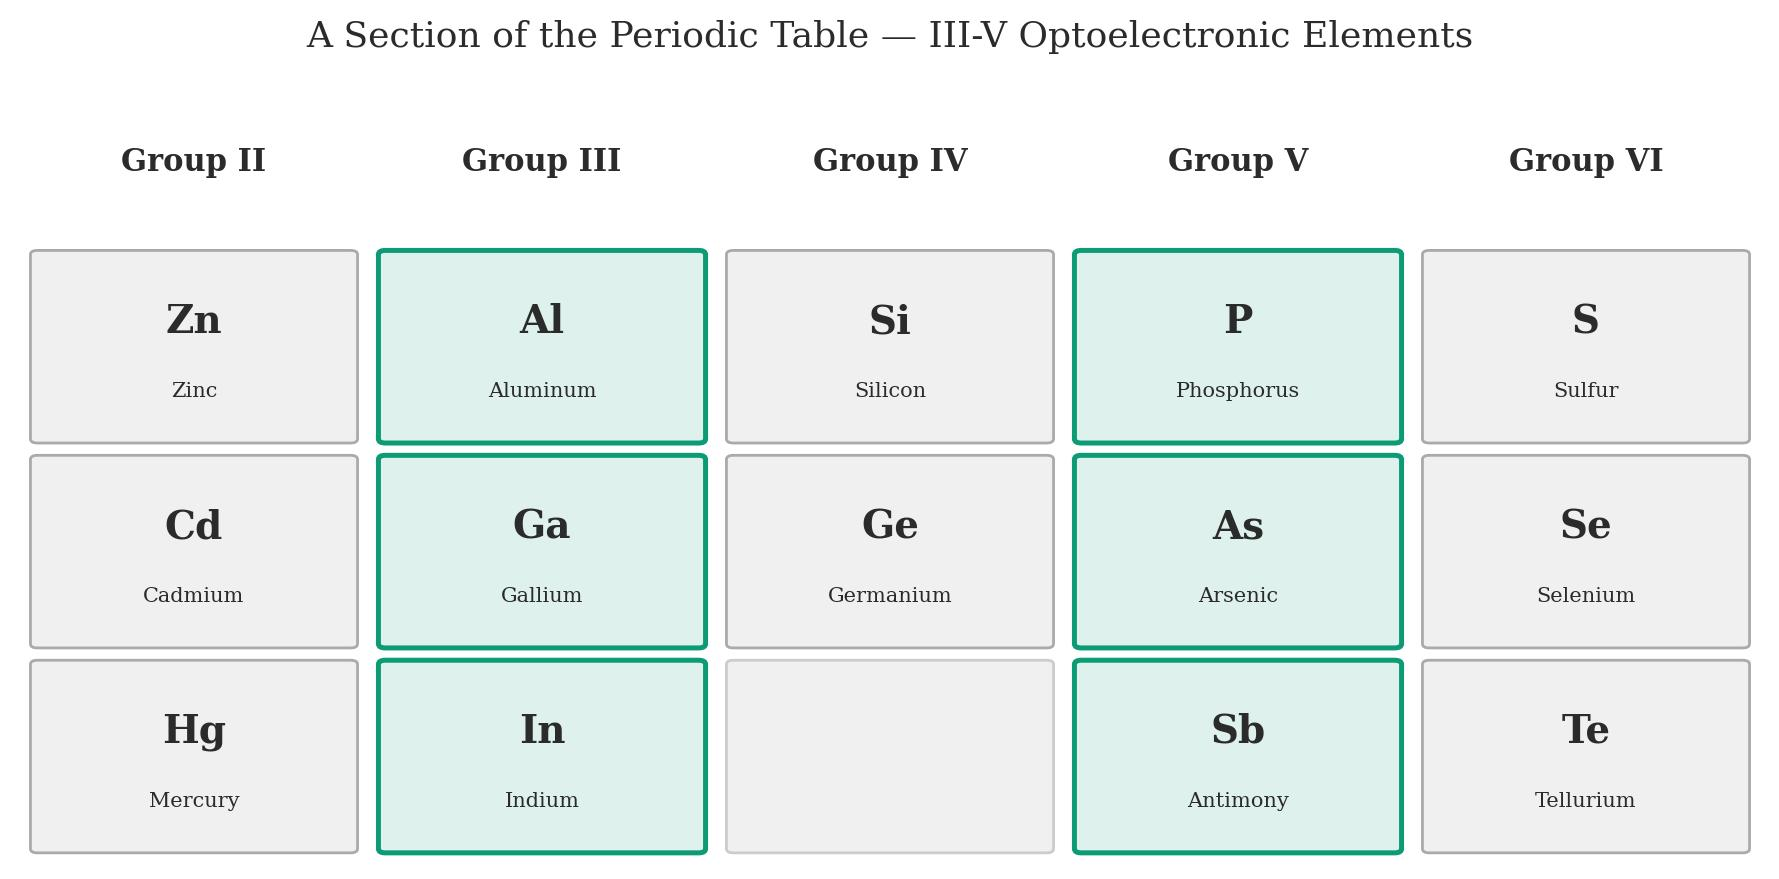
\includegraphics[width=0.6\textwidth]{Figures/Chapter 7/periodic_table_section.jpg}
    \caption{III-V Binary Semiconductor Periodic Table Section}
    \label{fig:periodic_table_section}
\end{figure}

Some key binary compounds at room temperature are:

\begin{center}
    \begin{tabular}{@{} l c c c @{}}
        \toprule
        \textbf{Material} & $E_g$ \textbf{(eV)} & $\lambda_g$ \textbf{($\mu$m)} & \textbf{Gap Type} \\
        \midrule
        GaAs              & 1.42                & 0.87                          & Direct            \\
        InP               & 1.35                & 0.92                          & Direct            \\
        InAs              & 0.36                & 3.5                           & Direct            \\
        GaSb              & 0.73                & 1.70                          & Direct            \\
        AlAs              & 2.16                & 0.57                          & Indirect          \\
        GaP               & 2.26                & 0.55                          & Indirect          \\
        Si                & 1.11                & 1.15                          & Indirect          \\
        \bottomrule
    \end{tabular}
\end{center}

\begin{figure}[H]
    \centering
    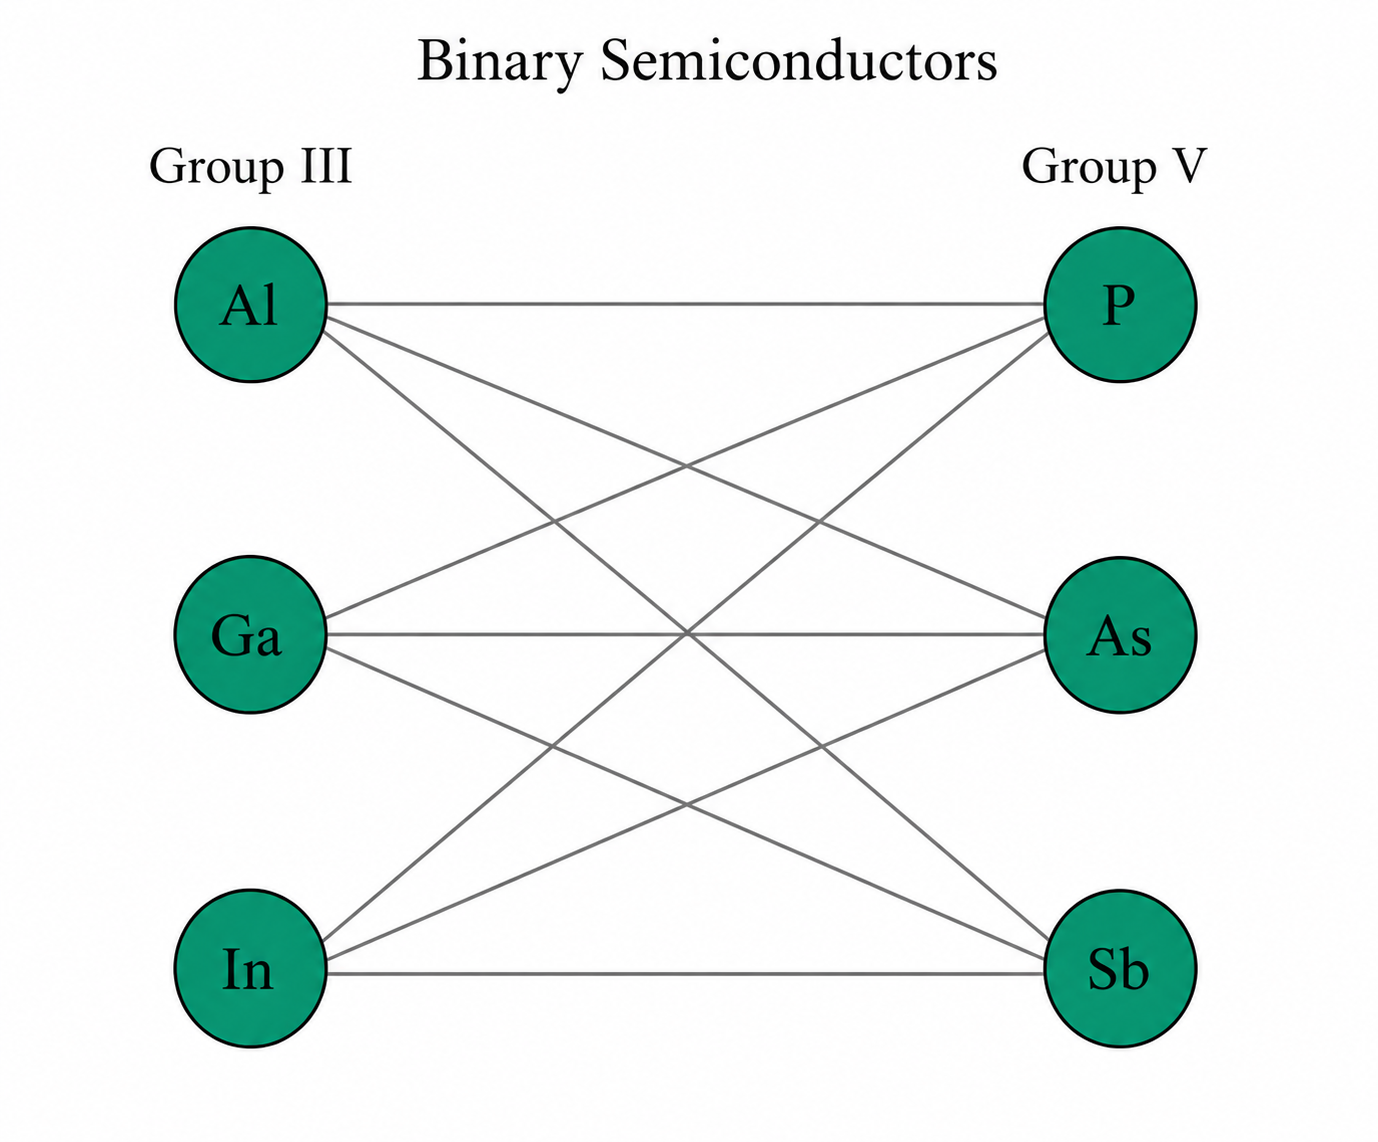
\includegraphics[width=0.6\textwidth]{Figures/Chapter 7/binary_semiconductor_connectivity_diagram.jpg}
    \caption{Binary Semiconductor Connectivity Diagram (Zincblende)}
    \label{fig:binary_semiconductor_connectivity_diagram}
\end{figure}

The bandgap is not a fixed constant — it shifts with temperature. For GaAs, the empirical Varshni formula gives:
\begin{equation*}
    E_g(\text{GaAs}) = 1.5216 - \frac{5.405 \times 10^{-4}\,T^2}{T + 204} \quad [\text{eV}]
\end{equation*}
and for InP:
\begin{equation*}
    E_g(\text{InP}) = 1.4206 - \frac{4.906 \times 10^{-4}\,T^2}{T + 327} \quad [\text{eV}]
\end{equation*}

The negative temperature coefficient means the bandgap shrinks as temperature rises — photon emission shifts to longer wavelengths at higher operating temperatures. This is one of the key reasons semiconductor laser output wavelength drifts with junction temperature, and it fundamentally couples thermal management to wavelength stability in practical devices.

\subsection{Ternary Semiconductors: Tuning the Bandgap}

No single binary compound can cover all the wavelength ranges required by applications. By mixing two Group-III elements with one Group-V element (or vice versa), we create ternary alloys whose bandgap and lattice constant can be continuously tuned by adjusting the composition fraction $x$.

To predict the properties of a ternary alloy, we use interpolation. The structural property—the lattice constant $a$—follows \textbf{Vegard's Law}, which states that the lattice constant is a strictly linear combination of the constituent binaries:
\begin{equation*}
    a\!\left(\text{Al}_x\text{Ga}_{1-x}\text{As}\right) = x\,a(\text{AlAs}) + (1-x)\,a(\text{GaAs})
\end{equation*}

However, the electronic property—the bandgap $E_g$—does not perfectly follow a linear average because the random distribution of alloy atoms slightly warps the crystal potential. We account for this physical warping by adding a nonlinear \textbf{bowing parameter} $C$:
\begin{equation*}
    E_g\!\left(\text{Al}_x\text{Ga}_{1-x}\text{As}\right) = x\,E_g(\text{AlAs}) + (1-x)\,E_g(\text{GaAs}) - C x(1-x)
\end{equation*}
For AlGaAs, the linear term gives approximately $1.424 + 1.247x\,\text{eV}$, and the bowing parameter $C$ is small, making the linear approximation acceptable for basic engineering estimates.

Specifically, the bandgap of the $\text{Al}_x\text{Ga}_{1-x}\text{As}$ alloy at room temperature is determined by the lowest of three conduction band valleys: the direct $\Gamma$ valley, the indirect $X$ valley, and the indirect $L$ valley. The energy of these valley minima relative to the valence band maximum as a function of the aluminum mole fraction $x$ are given by:
\begin{align*}
    E_g^\Gamma(x) &= 1.424 + 1.247x \quad [\text{eV}] \\
    E_g^X(x) &= 1.900 + 0.125x + 0.143x^2 \quad [\text{eV}] \\
    E_g^L(x) &= 1.708 + 0.642x \quad [\text{eV}]
\end{align*}
For small aluminum fractions, the direct $\Gamma$ valley is the lowest in energy, meaning AlGaAs is a direct-bandgap semiconductor. The direct-to-indirect crossover composition $x_c$ is determined by equating the energy of the direct $\Gamma$ valley and the indirect $X$ valley:
\begin{equation*}
    1.424 + 1.247x_c = 1.900 + 0.125x_c + 0.143x_c^2 \implies 0.143x_c^2 - 1.122x_c + 0.476 = 0
\end{equation*}
Solving this quadratic equation for the physical range $0 \le x_c \le 1$:
\begin{equation*}
    x_c = \frac{1.122 - \sqrt{(-1.122)^2 - 4(0.143)(0.476)}}{2(0.143)} \approx 0.45
\end{equation*}
For $x \le 0.45$, the bandgap is direct, which is a key requirement for efficient radiative recombination in optoelectronic devices. Above this threshold ($x > 0.45$), the material becomes an indirect-gap semiconductor.

The absolute critical constraint in heterostructure engineering is \textbf{lattice matching}. When we grow an epitaxial layer onto a substrate, the atoms of the new layer attempt to align with the existing substrate lattice. If their natural lattice constants $a$ differ, the newly grown layer experiences tremendous mechanical strain.
What happens physically? The layer can accommodate this elastic strain up to a certain \textbf{critical thickness} $h_c$. Below $h_c$, the layer is simply compressed or stretched (pseudomorphic growth). But if we grow the layer thicker than $h_c$, the accumulated strain energy becomes so massive that the crystal snaps. It violently relieves the stress by creating \textbf{misfit dislocations}—missing or extra half-planes of atoms at the interface. These broken atomic bonds create deep trap states in the middle of the bandgap, which act as aggressively efficient non-radiative recombination centres. This catastrophically reduces device efficiency, generates intense localized heat, and kills the device lifetime. As a rule of thumb, mismatch must be kept below $\sim 0.1\%$.

AlGaAs is the holy grail for near-infrared devices because GaAs and AlAs happen to have nearly identical lattice constants (they differ by less than $0.15\%$). According to Vegard's law, this means $\text{Al}_x\text{Ga}_{1-x}\text{As}$ is lattice-matched to GaAs for \emph{all} values of $x$ — the composition can be tuned freely across the full direct-gap range ($x \lesssim 0.45$) without ever crossing the critical thickness threshold for misfit dislocations. The resulting refractive index step between active and cladding layers is approximately:
\begin{equation*}
    n_\text{GaAs} - n_\text{AlGaAs} \approx 0.62x
\end{equation*}
which directly sets the waveguiding strength. Larger $x$ gives a bigger index step and stronger photon confinement, but also a larger bandgap discontinuity and stronger carrier confinement.

\begin{figure}[H]
    \centering
    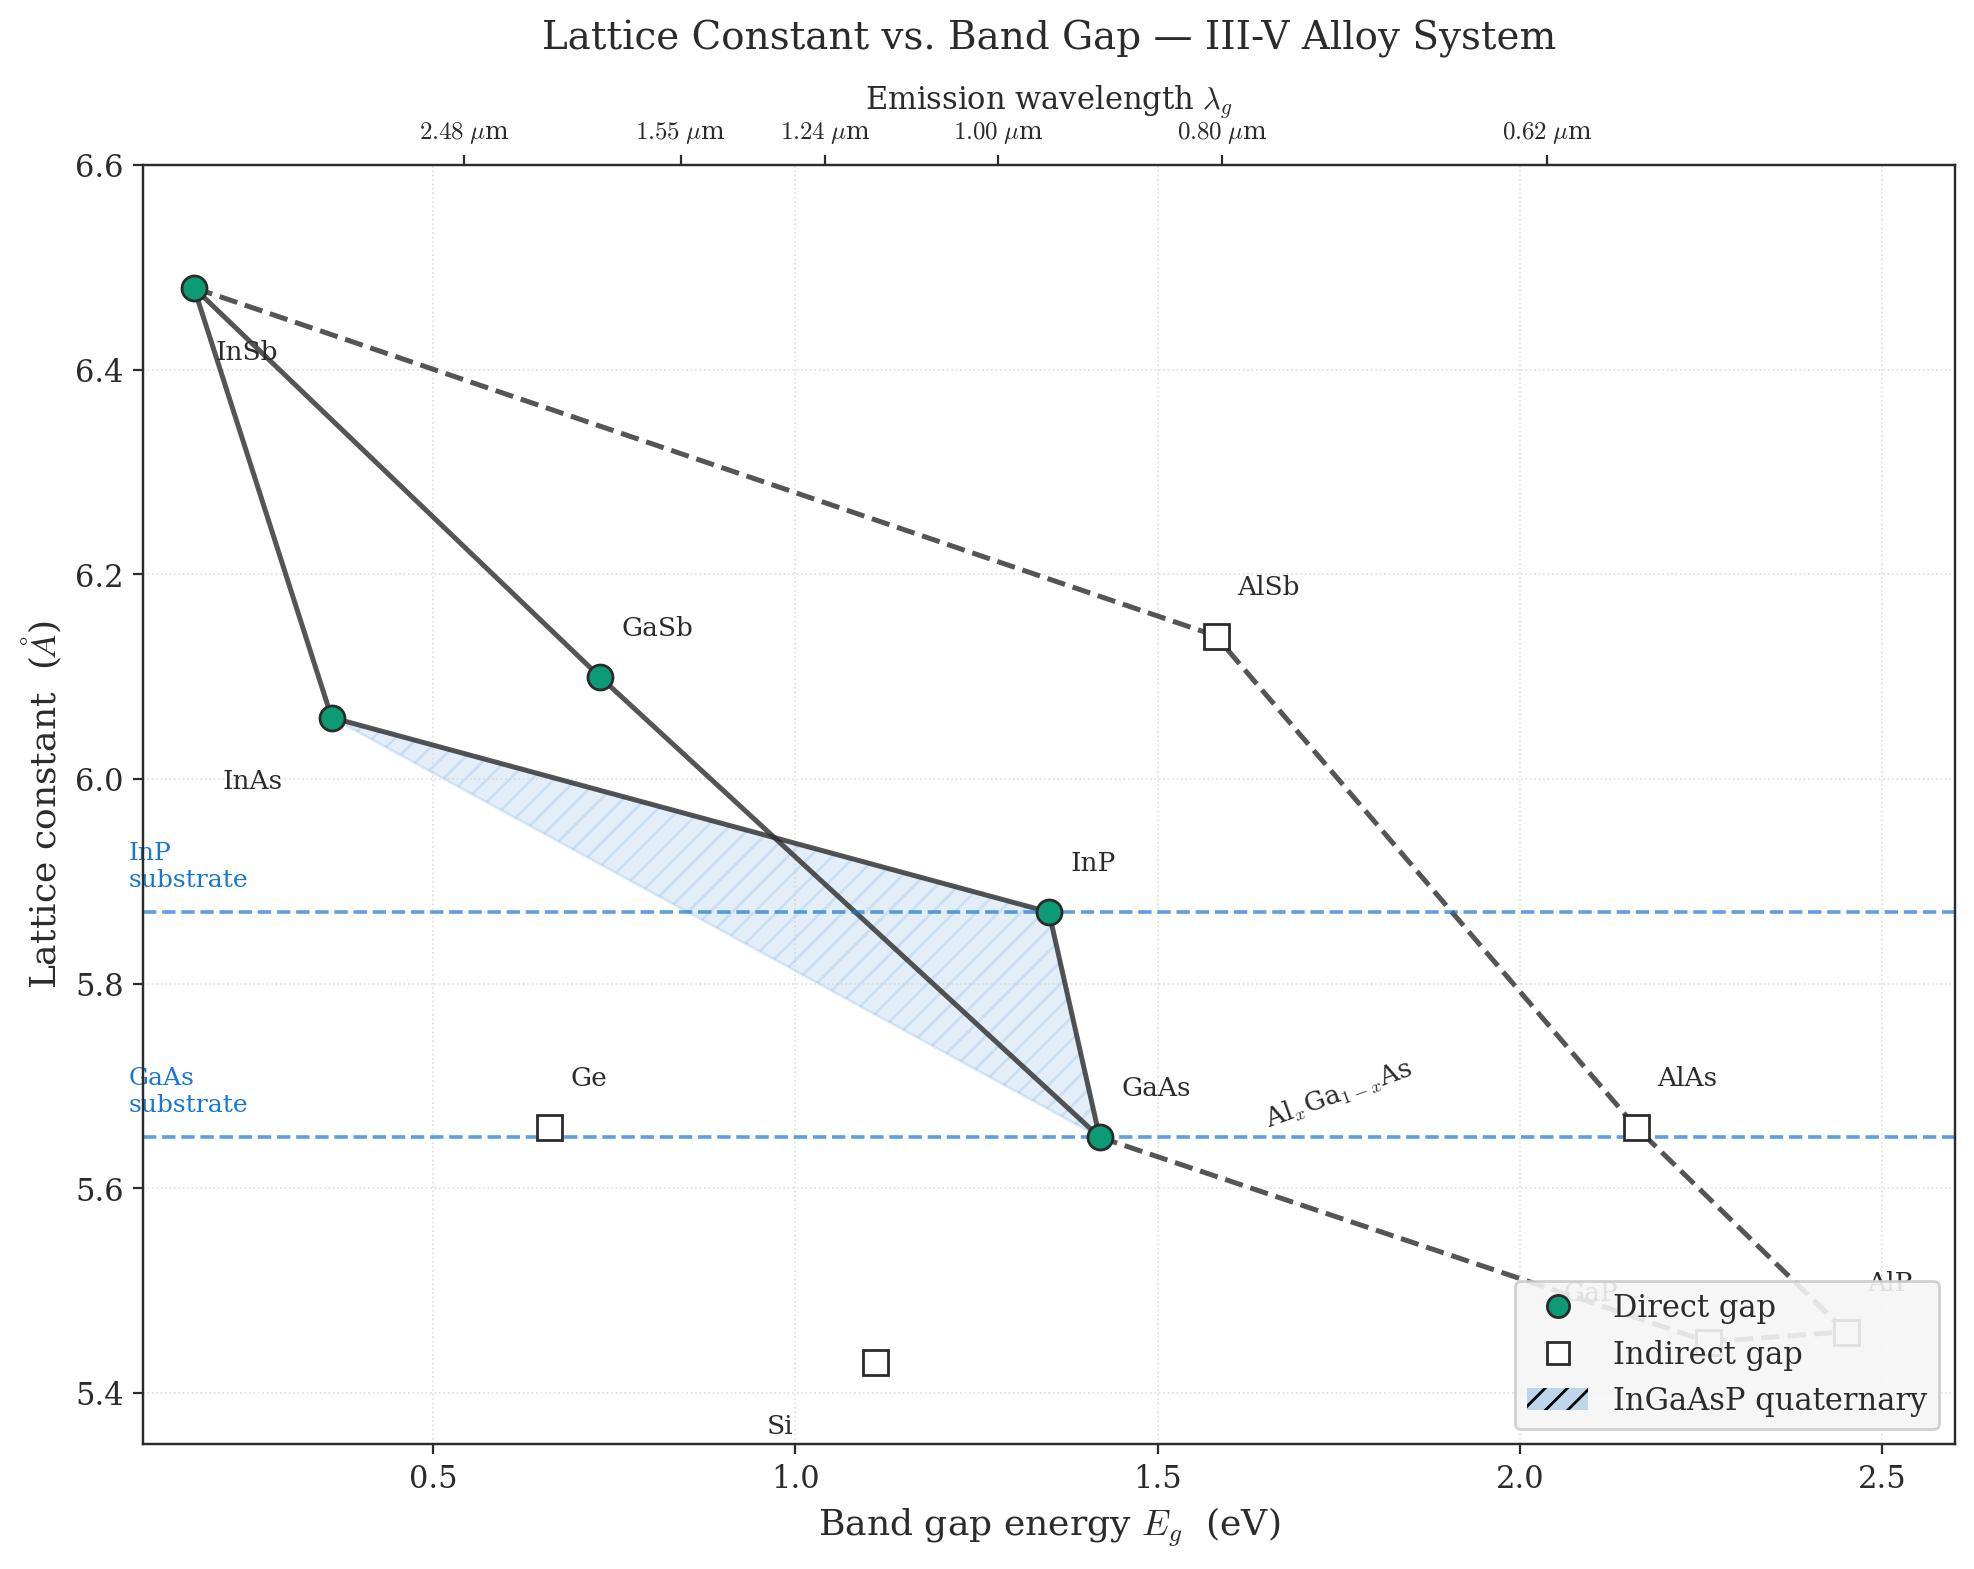
\includegraphics[width=0.6\textwidth]{Figures/Chapter 7/lattice_bandgap_alloy_map.jpg}
    \caption{Lattice Constant vs. Band Gap: Ternary Alloy Map}
    \label{fig:lattice_bandgap_alloy_map}
\end{figure}

\subsection{Quaternary Semiconductors: Decoupling Bandgap from Lattice Constant}

In a ternary alloy, adjusting $x$ to change the bandgap simultaneously changes the lattice constant. This limits design freedom: we can only choose compositions that are naturally lattice-matched to a given substrate. Quaternary alloys — using two Group-III and two Group-V elements — provide an extra degree of freedom that decouples the bandgap from the lattice constant. Both can be independently matched to a chosen substrate.

The most important quaternary system is In$_{1-x}$Ga$_x$As$_y$P$_{1-y}$ grown on InP substrates, where $x$ represents the Gallium mole fraction and $y$ represents the Arsenic mole fraction. To find its lattice constant, we apply a 2D bilinear interpolation (Vegard's law in two dimensions) across the four constituent binaries:
\begin{equation*}
    a(x,y) = (1-x)(1-y)\,a(\text{InP}) + x(1-y)\,a(\text{GaP}) + (1-x)y\,a(\text{InAs}) + xy\,a(\text{GaAs})
\end{equation*}
At $T = 300\text{ K}$, the lattice constants of the constituent binary materials are:
\begin{itemize}
    \item $a(\text{InP}) = 5.8687\,\text{\AA}$
    \item $a(\text{GaP}) = 5.4505\,\text{\AA}$
    \item $a(\text{InAs}) = 6.0584\,\text{\AA}$
    \item $a(\text{GaAs}) = 5.6533\,\text{\AA}$
\end{itemize}
To avoid misfit dislocations, we demand that the quaternary lattice constant matches that of the substrate: $a(x,y) = a(\text{InP})$. Expanding the interpolation formula yields:
\begin{align*}
    a(x,y) &= (1-x-y+xy)\,a(\text{InP}) + (x-xy)\,a(\text{GaP}) + (y-xy)\,a(\text{InAs}) + xy\,a(\text{GaAs}) \\
    &= a(\text{InP}) + x\,[a(\text{GaP}) - a(\text{InP})] + y\,[a(\text{InAs}) - a(\text{InP})] + xy\,[a(\text{GaAs}) - a(\text{GaP}) - a(\text{InAs}) + a(\text{InP})]
\end{align*}
Setting $a(x,y) = a(\text{InP})$ yields the condition:
\begin{equation*}
    x\,[a(\text{GaP}) - a(\text{InP})] + y\,[a(\text{InAs}) - a(\text{InP})] + xy\,[a(\text{GaAs}) - a(\text{GaP}) - a(\text{InAs}) + a(\text{InP})] = 0
\end{equation*}
Plugging in the numerical lattice constants:
\begin{gather*}
    x\,[5.4505 - 5.8687] + y\,[6.0584 - 5.8687] + xy\,[5.6533 - 5.4505 - 6.0584 + 5.8687] = 0 \\
    -0.4182x + 0.1897y + 0.0131xy = 0
\end{gather*}
Dividing by $0.1897$ to isolate $y$:
\begin{equation*}
    -2.2045x + y + 0.0691xy = 0 \implies y(1 + 0.0691x) = 2.2045x \implies y = \frac{2.2045x}{1 + 0.0691x}
\end{equation*}
Since $x \le 0.47$ for the composition range of interest, the term $0.0691x \le 0.032 \ll 1$, which allows us to neglect the second-order coupling term in the denominator. This yields the linear lattice-matching constraint:
\begin{equation*}
    y \approx 2.2x, \qquad x \lesssim 0.47
\end{equation*}

For the bandgap $E_g$, we similarly interpolate the four binaries, but we must also include bowing parameters for each of the ternary sub-systems to accurately account for crystal potential warping. The primary linear base is:
\begin{equation*}
    E_{g,\text{linear}} \approx (1-x)(1-y)\,E_g(\text{InP}) + x(1-y)\,E_g(\text{GaP}) + (1-x)y\,E_g(\text{InAs}) + xy\,E_g(\text{GaAs})
\end{equation*}
By applying the lattice-matching constraint $y \approx 2.2x$, we effectively remove one degree of freedom. This leaves one free parameter (say $y$, the Arsenic fraction) for continuously tuning the bandgap (and therefore the emission wavelength) while mechanically guaranteeing a defect-free interface. This specific family of alloys spans the precise energies needed for the $1.3\,\mu$m and $1.55\,\mu$m telecommunications windows, making it the bedrock of all long-haul fibre-optic sources.

% ------------------------------------------------------------------
\section{Heterostructure Operation: Injection Efficiency and Confinement}
% ------------------------------------------------------------------

\subsection{Injection Efficiency at a Single Heterojunction}

When we forward-bias a p-n junction to inject carriers into our active region, we want to inject carriers of one type (say, electrons) as efficiently as possible while suppressing the counter-injection of the opposite carrier type (holes). The parameter that measures our success in doing this is the injection efficiency, which represents the fraction of the total junction current carried by the desired carrier type:
\begin{keyresult}
    \begin{equation}
        \eta_j = \frac{J_e}{J_e + J_h}
    \end{equation}
\end{keyresult}
where:
$\eta_j$: injection efficiency of the junction
$J_e$: electron current density injected across the junction
$J_h$: hole current density counter-injected across the junction

If we want the injection efficiency to approach unity, we must make the ratio of the unwanted hole current to the desired electron current as close to zero as possible. To see how this works, we can rearrange this expression by dividing both the numerator and the denominator by the electron current density:
\begin{equation*}
    \eta_j = \frac{\dfrac{J_e}{J_e}}{\dfrac{J_e}{J_e} + \dfrac{J_h}{J_e}}
\end{equation*}
which simplifies directly to our working relation:
\begin{equation}
    \eta_j = \frac{1}{1 + \dfrac{J_h}{J_e}} \tag{I}
\end{equation}

This shows that minimizing the current ratio $J_h / J_e$ is the absolute key to maximizing our injection efficiency. Let's analyze the two types of junctions to see how they perform.

In a traditional homojunction, both sides are made of the same semiconductor material, meaning they share the same bandgap. To find the ratio of the minority carrier diffusion currents crossing the depletion region under a forward bias $V$, we solve the steady-state diffusion equations at the boundaries of the depletion region. The electron current density injected into the p-side is:
\begin{equation*}
    J_e = \frac{e D_e n_{p0}}{L_e} \left[ \exp\left(\frac{eV}{k_B T}\right) - 1 \right] = \frac{e D_e n_i^2}{L_e N_A} \left[ \exp\left(\frac{eV}{k_B T}\right) - 1 \right]
\end{equation*}
where $n_{p0} = n_i^2/N_A$ is the minority electron density at equilibrium in the p-side, $D_e$ is the electron diffusion coefficient, and $L_e$ is the electron diffusion length. Similarly, the hole current density injected into the n-side is:
\begin{equation*}
    J_h = \frac{e D_h p_{n0}}{L_h} \left[ \exp\left(\frac{eV}{k_B T}\right) - 1 \right] = \frac{e D_h n_i^2}{L_h N_D} \left[ \exp\left(\frac{eV}{k_B T}\right) - 1 \right]
\end{equation*}
where $p_{n0} = n_i^2/N_D$ is the minority hole density at equilibrium in the n-side, $D_h$ is the hole diffusion coefficient, and $L_h$ is the hole diffusion length. Taking the ratio of these current densities yields:
\begin{equation*}
    \left(\frac{J_h}{J_e}\right)_{\text{homo}} = \frac{\dfrac{e D_h n_i^2}{L_h N_D}}{\dfrac{e D_e n_i^2}{L_e N_A}} = \frac{D_h}{D_e} \cdot \frac{L_e}{L_h} \cdot \frac{N_A}{N_D}
\end{equation*}
where:
$D_h$: hole diffusion coefficient on the n-side
$D_e$: electron diffusion coefficient on the p-side
$L_h$: hole diffusion length on the n-side
$L_e$: electron diffusion length on the p-side
$N_A$: acceptor doping concentration on the p-side
$N_D$: donor doping concentration on the n-side

Substituting this ratio into our general efficiency equation \textup{(I)} yields the homojunction injection efficiency:
\begin{equation*}
    \eta_{j,\text{homo}} = \frac{1}{1 + \dfrac{D_h L_e N_A}{D_e L_h N_D}}
\end{equation*}
Under ordinary conditions, the diffusion coefficients and lengths are fixed by the material quality, leaving us with only the doping ratio $N_A / N_D$ as an active design handle. To make the ratio $J_h / J_e$ small (and thus $\eta_j \approx 1$), we are forced to dope the n-side far more heavily than the p-side ($N_D \gg N_A$). This imposes a severe constraint on device design: extremely high doping levels introduce non-radiative defects, cause bandgap narrowing, and increase free-carrier absorption, which degrades performance.

Now let's see how a single heterojunction — where we join a wide-bandgap n-type semiconductor (the emitter) to a narrow-bandgap p-type semiconductor (the active region) — completely breaks this bottleneck. The difference in bandgaps, $\Delta E_g = E_{g,\text{wide}} - E_{g,\text{narrow}}$, alters the intrinsic carrier concentrations on both sides of the junction:
\begin{align*}
    n_{i,\text{wide}}^2 &= N_{C,\text{wide}} N_{V,\text{wide}} \exp\left(-\frac{E_{g,\text{wide}}}{k_B T}\right) \\
    n_{i,\text{narrow}}^2 &= N_{C,\text{narrow}} N_{V,\text{narrow}} \exp\left(-\frac{E_{g,\text{narrow}}}{k_B T}\right)
\end{align*}
Because the electron injection current $J_e$ is determined by the parameters of the narrow-gap p-type region, and the hole injection current $J_h$ is determined by the parameters of the wide-gap n-type region, their ratio becomes:
\begin{equation*}
    \left(\frac{J_h}{J_e}\right)_{\text{hetero}} = \frac{D_h}{D_e} \cdot \frac{L_e}{L_h} \cdot \frac{N_A}{N_D} \cdot \left(\frac{n_{i,\text{wide}}^2}{n_{i,\text{narrow}}^2}\right)
\end{equation*}
Substituting the expressions for the intrinsic concentrations:
\begin{equation*}
    \frac{n_{i,\text{wide}}^2}{n_{i,\text{narrow}}^2} = \left(\frac{N_{C,\text{wide}} N_{V,\text{wide}}}{N_{C,\text{narrow}} N_{V,\text{narrow}}}\right) \exp\left(-\frac{E_{g,\text{wide}} - E_{g,\text{narrow}}}{k_B T}\right)
\end{equation*}
Assuming that the ratio of the effective densities of states is approximately 1, we get:
\begin{keyresult}
    \begin{equation}
        \left(\frac{J_h}{J_e}\right)_{\text{hetero}} \approx \frac{D_h}{D_e} \cdot \frac{L_e}{L_h} \cdot \frac{N_A}{N_D} \cdot \exp\!\left(-\frac{\Delta E_g}{k_B T}\right)
    \end{equation}
\end{keyresult}
where:
$\Delta E_g$: bandgap difference between the wider cladding layer and the narrower active layer ($E_{g,\text{wide}} - E_{g,\text{narrow}}$)
$k_B$: Boltzmann constant
$T$: absolute temperature

The addition of the exponential factor $\exp(-\Delta E_g / k_B T)$ is an absolute game-changer. Let's look at a concrete example to see just how dominant this factor is. Suppose we have a bandgap difference of $\Delta E_g = 0.3\text{ eV}$ (which is easily achieved in the GaAs/Al$_x$Ga$_{1-x}$As system). At room temperature ($T = 300\text{ K}$), the thermal voltage is $k_B T \approx 0.0259\text{ eV}$. Plugging these values into the exponential factor:
\begin{equation*}
    \exp\!\left(-\frac{\Delta E_g}{k_B T}\right) = \exp\!\left(-\frac{0.3}{0.0259}\right) \approx 9.3 \times 10^{-6}
\end{equation*}
This means that the unwanted hole injection is suppressed by more than five orders of magnitude! Because of this massive exponential suppression, the ratio $J_h / J_e$ becomes negligible, forcing the heterojunction injection efficiency $\eta_j$ to approach virtually 100\%:
\begin{equation*}
    \eta_j \approx 1
\end{equation*}

The physical takeaway here is that the heterojunction introduces the bandgap difference $\Delta E_g$ as a completely new thermodynamic degree of freedom. We no longer have to rely on highly asymmetric doping ($N_D \gg N_A$) to get efficient injection. In fact, we can now choose the doping levels to optimize other properties — such as minimizing the series resistance or reducing free-carrier absorption — while still maintaining nearly perfect injection efficiency. This simple design freedom is the primary reason why heterostructure devices are so incredibly efficient.

The current components across a typical p-n junction are shown in the sketch below. Notice how the electron flow from the wider-gap n-side dominates the total carrier transport across the interface.

\begin{figure}[H]
    \centering
    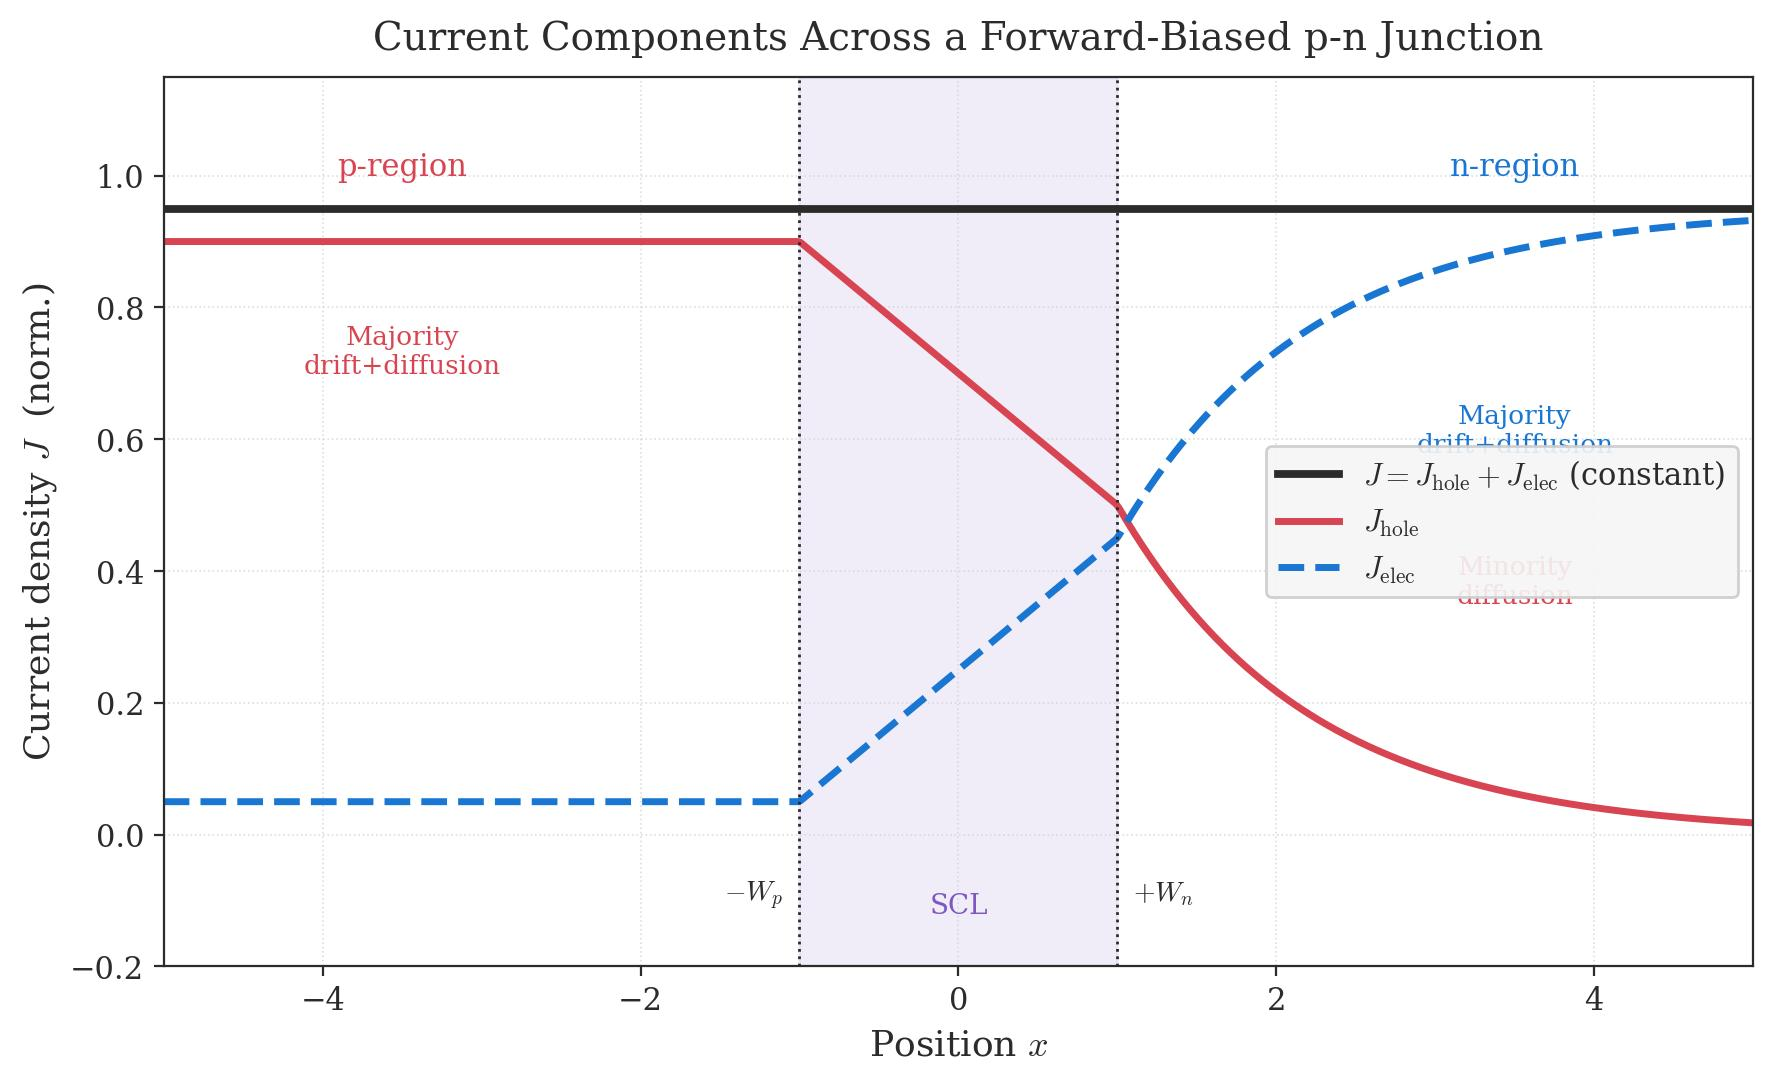
\includegraphics[width=0.6\textwidth]{Figures/Chapter 7/junction_current_components.jpg}
    \caption{Current Components Across a p-n Junction}
    \label{fig:junction_current_components}
\end{figure}

For a double heterostructure, injecting a wide-gap cladding on both sides of the narrow-gap active layer means that once carriers cross into the active region, the potential barriers on both sides prevent them from escaping. There is no longer a competing diffusion current flowing out into the bulk — all the injected current contributes to recombination within the active layer.

\subsection{Carrier Density Enhancement in the DH Structure}

We can quantify precisely how much better the DH structure is at building up carrier density for a given injected current. In the long p-side of a standard single junction, the steady-state diffusion of excess electrons $\Delta n(x)$ is governed by $D_e \frac{d^2 \Delta n}{dx^2} - \frac{\Delta n}{\tau} = 0$. With boundary conditions $\Delta n(0)$ at the depletion edge ($x=0$) and $\Delta n(\infty) = 0$, the spatial profile is:
\begin{equation*}
    \Delta n(x) = \Delta n(0) \exp\left(-\frac{x}{L_e}\right)
\end{equation*}
where $L_e = \sqrt{D_e \tau}$ is the electron diffusion length. The injected current density at the interface is purely due to diffusion:
\begin{equation*}
    J = e D_e \left. \frac{d \Delta n}{dx} \right|_{x=0} = \frac{e D_e \Delta n(0)}{L_e} \implies \Delta n(0) = \frac{J L_e}{e D_e}
\end{equation*}
Using $D_e = L_e^2 / \tau$, the surface excess carrier density simplifies to:
\begin{equation*}
    \Delta n(0) = \frac{J \tau}{e L_e}
\end{equation*}
For a thin DH active layer of thickness $d \ll L_e$, the potential barriers at the boundaries reflect the carriers, keeping them confined. Thus, the carrier density $\Delta N$ is approximately uniform across $d$. The steady-state continuity equation requires:
\begin{equation*}
    \frac{J}{ed} = \frac{\Delta N}{\tau} \implies \Delta N = \frac{J \tau}{e d}
\end{equation*}
Taking the ratio of the carrier density in the DH active region to the peak surface carrier density in the homojunction under the same injected current density $J$:
\begin{equation*}
    \frac{\Delta N}{\Delta n(0)} = \frac{\dfrac{J\tau}{ed}}{\dfrac{J\tau}{eL_e}} = \frac{L_e}{d}
\end{equation*}

Since $L_e \sim 1\,\mu$m and $d \sim 0.1\,\mu$m for a well-designed DH laser, the carrier density in the active region is enhanced by a factor of $L_e/d \sim 10$ compared to a homojunction for the same injected current. This is the quantitative explanation for why DH lasers achieve much lower threshold currents.

\subsection{Single-Mode Waveguide Condition}

The active layer must also confine the optical mode. We treat the heterostructure as a symmetric slab waveguide with core thickness $d$, core index $n_1$, and cladding index $n_2$ ($n_1 > n_2$). Inside the core ($|x| < d/2$), the fields propagate as waves with transverse wave number $k_x = \sqrt{n_1^2 k_0^2 - \beta^2}$, where $k_0 = 2\pi/\lambda_0$ and $\beta$ is the propagation constant. In the cladding ($|x| > d/2$), the fields decay exponentially with decay constant $\gamma_x = \sqrt{\beta^2 - n_2^2 k_0^2}$. These parameters satisfy:
\begin{equation*}
    k_x^2 + \gamma_x^2 = (n_1^2 - n_2^2) k_0^2
\end{equation*}
Matching the boundary conditions (continuity of tangential $E$ and $H$ fields) at the core-cladding interfaces $x = \pm d/2$ leads to the guided mode eigenvalue equations. For transverse electric (TE) modes:
\begin{itemize}
    \item Even modes: $k_x \tan\left(k_x \dfrac{d}{2}\right) = \gamma_x$
    \item Odd modes: $k_x \cot\left(k_x \dfrac{d}{2}\right) = -\gamma_x$
\end{itemize}
The fundamental even mode ($TE_0$) has no cutoff frequency. The first higher-order mode is the odd $TE_1$ mode, which reaches its cutoff condition when it is no longer bound in the cladding, corresponding to $\gamma_x \to 0$. Substituting $\gamma_x = 0$ into the odd mode eigenvalue equation:
\begin{equation*}
    k_x \cot\left(k_x \frac{d}{2}\right) = 0 \implies k_x \frac{d}{2} = \frac{\pi}{2}
\end{equation*}
Since $\gamma_x = 0$, we have $k_x = k_0\sqrt{n_1^2 - n_2^2} = \frac{2\pi}{\lambda_0}\sqrt{n_1^2 - n_2^2}$. Substituting this into the cutoff relation gives the maximum thickness $d_{\text{max}}$ for single-mode operation:
\begin{equation*}
    \left(\frac{2\pi}{\lambda_0}\sqrt{n_1^2 - n_2^2}\right) \frac{d_{\text{max}}}{2} = \frac{\pi}{2} \implies d_{\text{max}} = \frac{\lambda_0}{2\sqrt{n_1^2 - n_2^2}}
\end{equation*}
By defining the normalized frequency parameter $V$ using the full thickness $d$:
\begin{keyresult}
    \begin{equation}
        V = \frac{2\pi d}{\lambda_0}\sqrt{n_1^2 - n_2^2}
    \end{equation}
\end{keyresult}
the condition $d < d_{\text{max}}$ for single-transverse-mode operation translates directly to:
\begin{equation*}
    V < \pi
\end{equation*}

This reveals an important design trade-off: reducing $d$ below $d_\text{max}$ guarantees single-mode operation and also reduces the threshold current (higher carrier density for same $J$), but it simultaneously reduces the optical confinement factor $\Gamma$ — a thinner waveguide confines less of the mode power in the gain region. The modal gain $\gamma_\text{modal} = \Gamma\,\gamma_\text{med}$ therefore drops as $d$ decreases below a critical value, ultimately raising the threshold instead of lowering it. There is an optimal active layer thickness that minimises the threshold current density, and it is typically in the range $d \approx 50$--$200\,\text{nm}$ for GaAs-based DH lasers.

\begin{figure}[H]
    \centering
    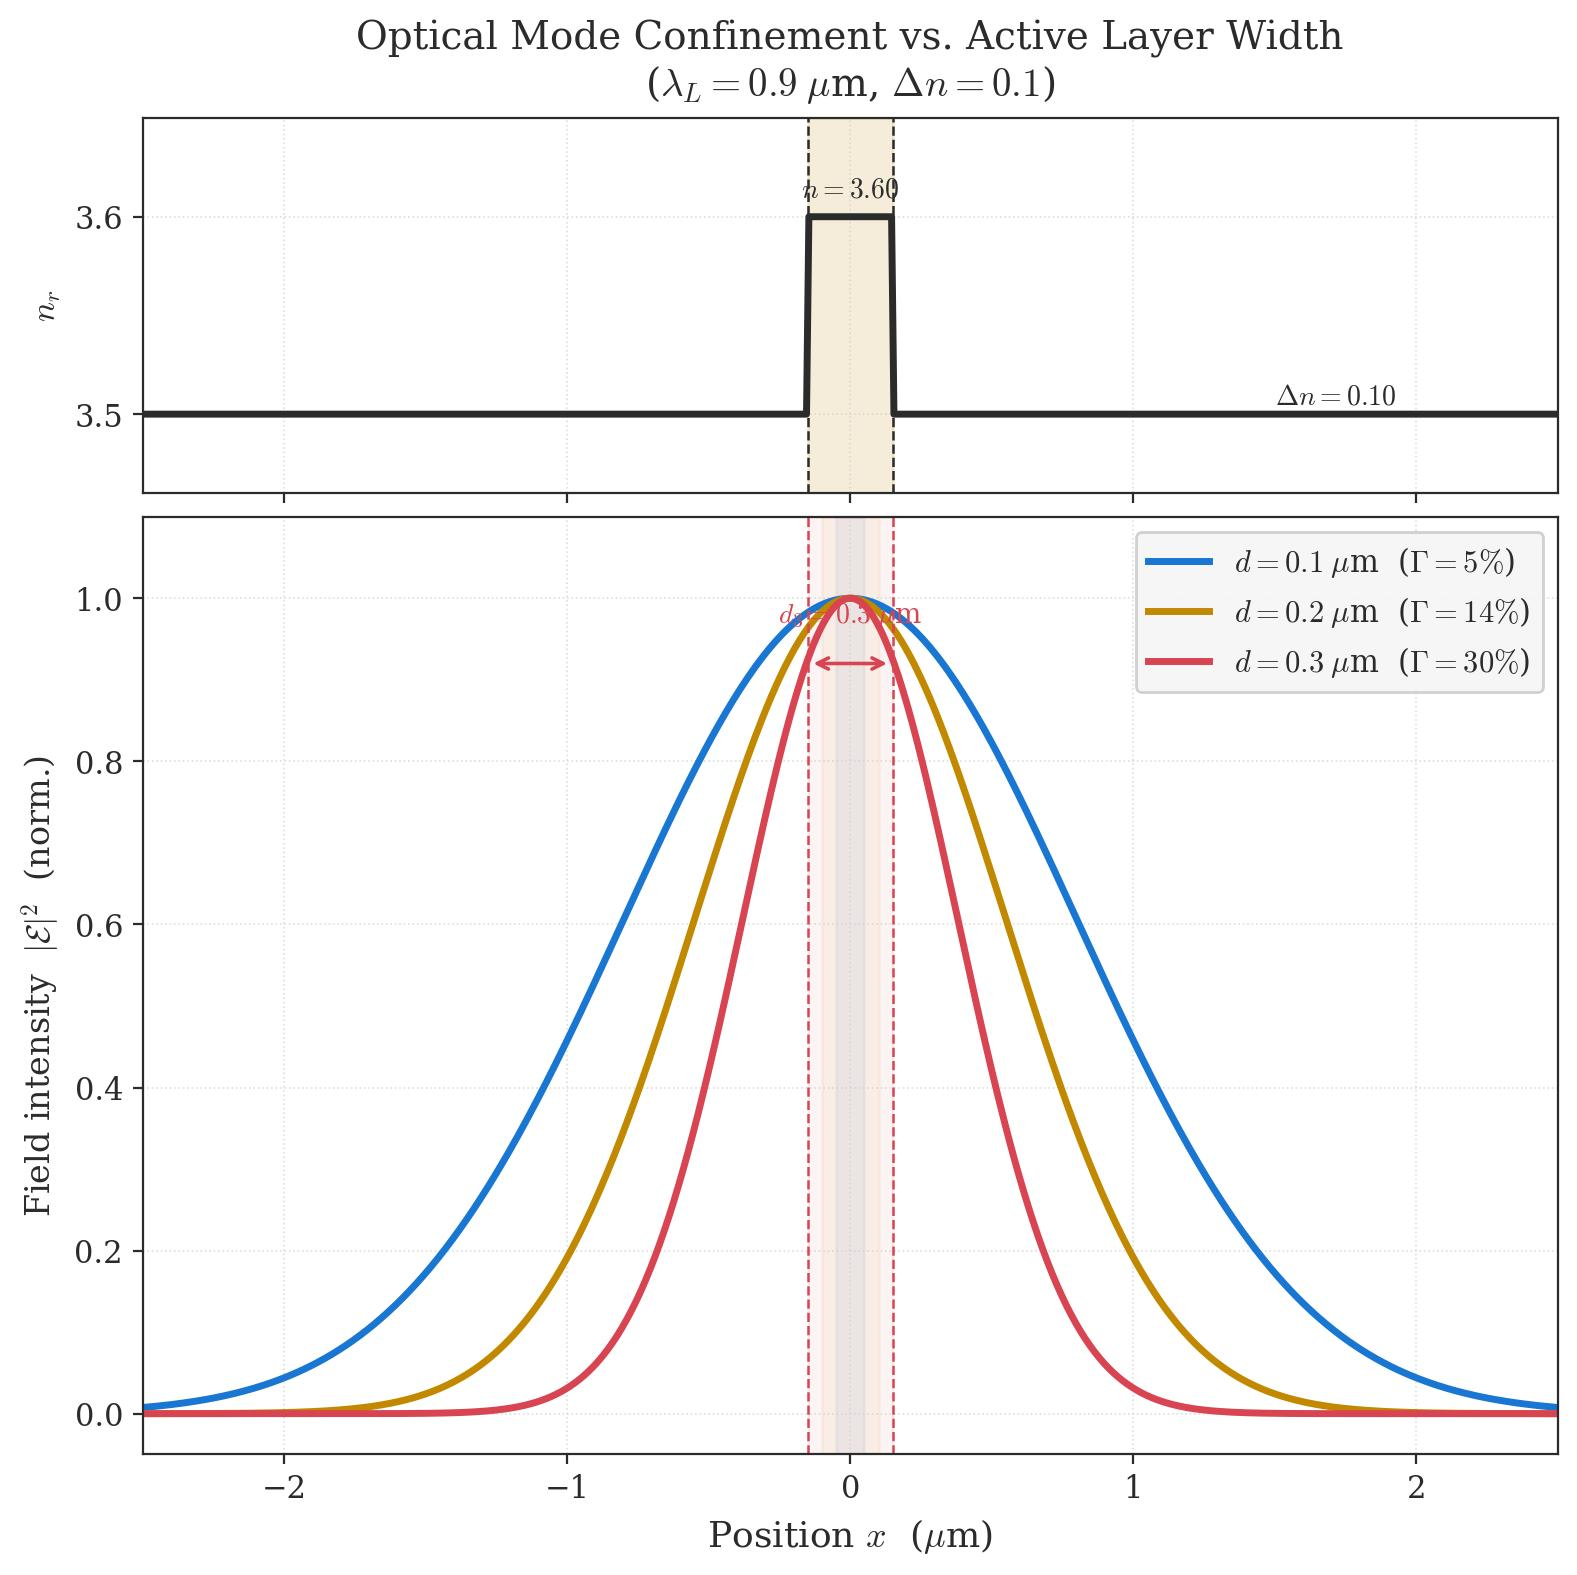
\includegraphics[width=0.6\textwidth]{Figures/Chapter 7/confinement_vs_thickness.jpg}
    \caption{Optical Confinement Factor vs. Active Layer Thickness}
    \label{fig:confinement_vs_thickness}
\end{figure}

% ------------------------------------------------------------------
\section{The Carrier Rate Equation}
% ------------------------------------------------------------------

\subsection{Generation: Current Injection}

We now have all the ingredients to write down the complete dynamical equation governing the carrier population inside the active region. The rate of change of carrier density $N$ has three contributions: injection from the external current, spontaneous and non-radiative recombination, and stimulated emission consuming carriers to produce coherent photons.

To derive this term, we start from the charge conservation represented by the electron continuity equation:
\begin{equation*}
    \frac{\partial N}{\partial t} = -\frac{1}{e} \nabla \cdot \mathbf{J}_e + G - R
\end{equation*}
Integrating the current divergence term over the volume $V = A \cdot d$ of the active region, where $A$ is the junction area and $d$ is the active layer thickness:
\begin{equation*}
    \int_V \frac{\partial N}{\partial t} dV = -\frac{1}{e} \int_V \nabla \cdot \mathbf{J}_e dV = -\frac{1}{e} \oint_S \mathbf{J}_e \cdot d\mathbf{A}
\end{equation*}
Under the assumption of uniform injection across area $A$, the surface integral of the current density equals the net current entering the active layer $I = J \cdot A$. Assuming the carrier density $N$ is spatially uniform:
\begin{equation*}
    A d \left.\frac{dN}{dt}\right|_\text{gen} = \frac{I}{e} = \frac{J A}{e}
\end{equation*}
Dividing both sides by the active volume $A d$ gives the generation rate per unit volume:
\begin{equation*}
    \left.\frac{dN}{dt}\right|_\text{gen} = \frac{J}{ed}
\end{equation*}
where $e$ is the elementary charge and $d$ is the active layer thickness. This term simply counts how many electron-hole pairs per unit volume per second are supplied by the external current.

\subsection{Recombination: Three Mechanisms}

Carriers are consumed by three physically distinct recombination processes, each with a different microscopic origin and a different dependence on carrier density $N$:

\textbf{1. Shockley-Read-Hall (SRH) recombination} is a single-carrier, trap-assisted process. An electron or hole is captured by a mid-gap defect state (a lattice imperfection or impurity), which then captures the complementary carrier. No photon is emitted — the energy is released as heat (phonons). The rate scales linearly with carrier density:
\begin{equation*}
    R_\text{SRH} = AN
\end{equation*}
where $A$ (s$^{-1}$) is the SRH coefficient, proportional to the defect density. This is the dominant recombination channel in indirect-gap materials like silicon, where radiative transitions are phonon-assisted and therefore slow — $\tau_r \sim 10\,\text{ms}$ in Si compared to $\tau_r \sim 100\,\text{ns}$ in GaAs. Minimising $A$ through careful crystal growth and surface passivation is essential for high-efficiency LEDs.

\textbf{2. Bimolecular (radiative) recombination} is the direct band-to-band process that produces a photon. An electron and a hole meet, annihilate, and emit a photon with energy close to $E_g$. This process requires \emph{both} an electron and a hole, so its rate scales as $N^2$ (assuming the electron and hole densities are equal, i.e., $n = p = N$ under equal injection):
\begin{equation*}
    R_\text{rad} = BN^2
\end{equation*}
where $B$ (m$^3$/s) is the bimolecular recombination coefficient. For GaAs, $B \approx 10^{-16}\,\text{m}^3/\text{s}$ at room temperature. This is the channel that drives LED emission and laser gain.

\textbf{3. Auger recombination} is a three-particle process. An electron-hole pair recombines, but instead of emitting a photon, the released energy is transferred to a third carrier (either an electron or a hole) which is kicked to a higher energy state and subsequently thermalises back. The rate scales as $N^3$:
\begin{equation*}
    R_\text{Auger} = CN^3
\end{equation*}
where $C$ (m$^6$/s) is the Auger coefficient. Auger recombination is the dominant efficiency-limiting mechanism at high carrier densities and at elevated temperatures, and is a major challenge for long-wavelength lasers ($\lambda > 1.3\,\mu$m) where $C$ is large.

The total volumetric recombination rate combining all three mechanisms is:
\begin{keyresult}
    \begin{equation}
        R = AN + BN^2 + CN^3
    \end{equation}
\end{keyresult}

\begin{figure}[H]
    \centering
    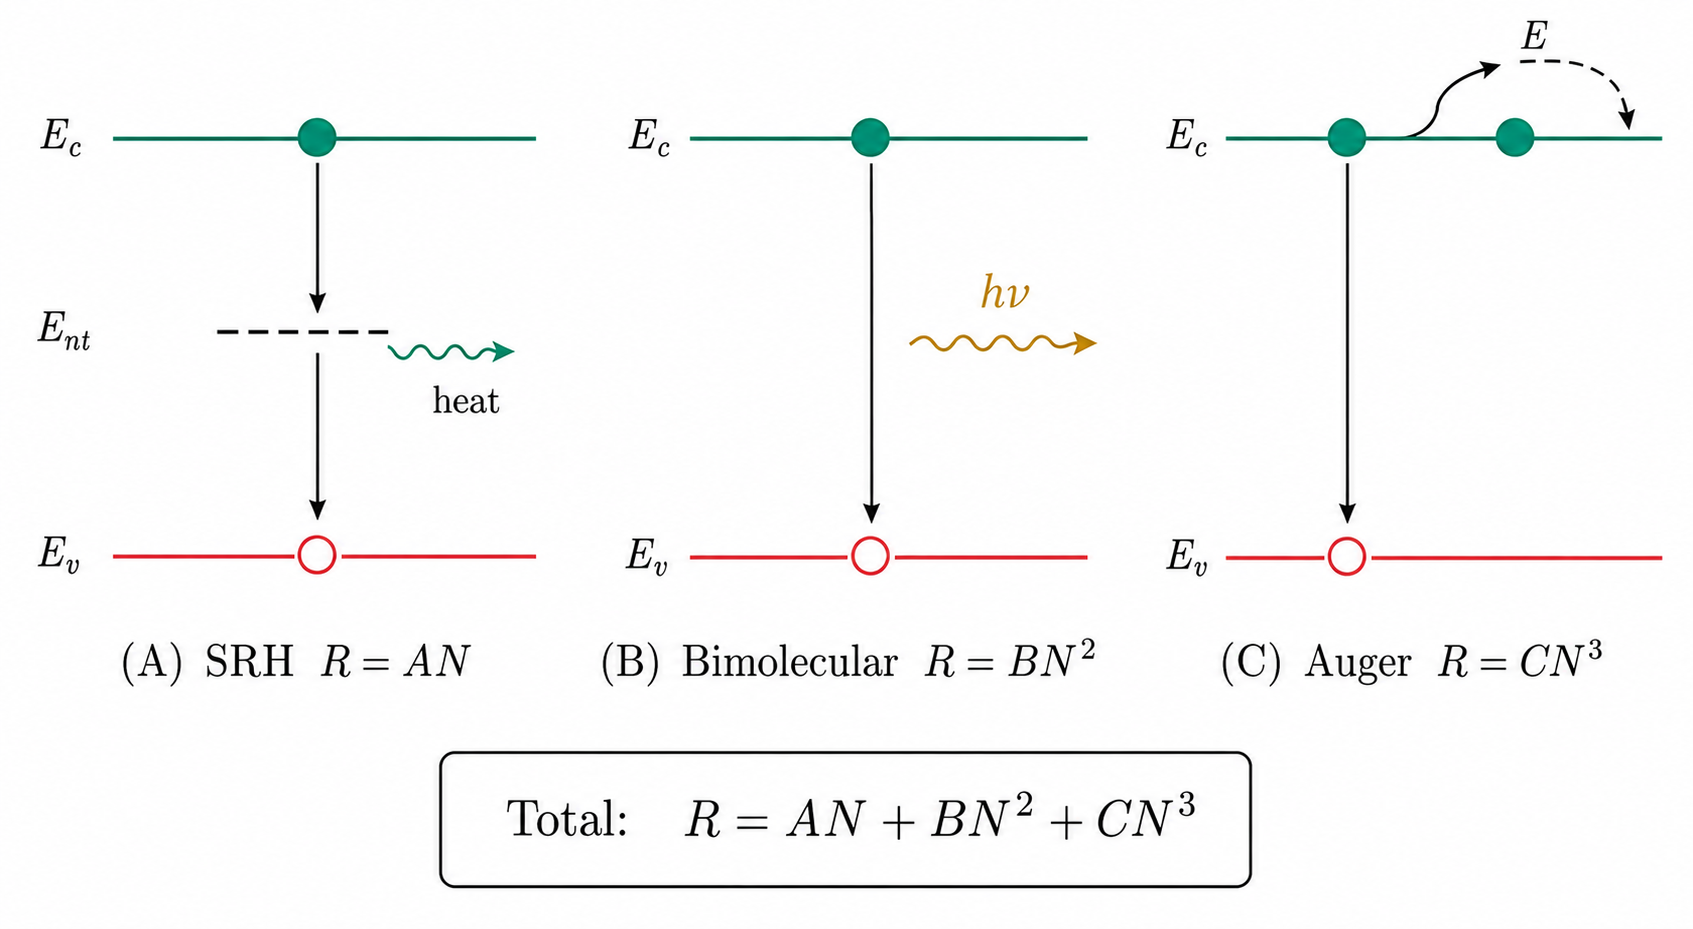
\includegraphics[width=0.7\textwidth]{Figures/Chapter 7/carrier_recombination_mechanisms.jpg}
    \caption{Carrier Recombination Mechanisms}
    \label{fig:carrier_recombination_mechanisms}
\end{figure}

\subsection{Carrier Lifetime and Internal Quantum Efficiency}

The total recombination rate $R$ is the sum of the three independent, parallel processes:
\begin{equation*}
    R = R_{\text{SRH}} + R_{\text{rad}} + R_{\text{Auger}} = AN + BN^2 + CN^3
\end{equation*}
We define a characteristic lifetime $\tau_i$ for each process by expressing the rate as $N/\tau_i$:
\begin{itemize}
    \item SRH lifetime: $\tau_{\text{SRH}} = \dfrac{1}{A}$
    \item Radiative lifetime: $\tau_r = \dfrac{1}{BN}$
    \item Auger lifetime: $\tau_{\text{Auger}} = \dfrac{1}{CN^2}$
\end{itemize}
Substituting these into the total recombination rate:
\begin{equation*}
    R = \frac{N}{\tau_{\text{SRH}}} + \frac{N}{\tau_r} + \frac{N}{\tau_{\text{Auger}}} = N \left( \frac{1}{\tau_{\text{SRH}}} + \frac{1}{\tau_r} + \frac{1}{\tau_{\text{Auger}}} \right)
\end{equation*}
Since the total carrier lifetime $\tau$ is defined implicitly by $R = N/\tau$, we have:
\begin{equation*}
    \frac{1}{\tau} = \frac{1}{\tau_r} + \left( \frac{1}{\tau_{\text{SRH}}} + \frac{1}{\tau_{\text{Auger}}} \right)
\end{equation*}
Grouping the non-radiative channels into a single non-radiative lifetime $\tau_{nr}$ defined by $\frac{1}{\tau_{nr}} = A + CN^2$:
\begin{keyresult}
    \begin{equation}
        \frac{1}{\tau} = \frac{1}{\tau_r} + \frac{1}{\tau_{nr}}
    \end{equation}
\end{keyresult}
The internal quantum efficiency $\eta_{\text{int}}$ represents the fraction of total recombination events that produce a radiative photon:
\begin{equation*}
    \eta_{\text{int}} = \frac{R_{\text{rad}}}{R} = \frac{BN^2}{AN + BN^2 + CN^3} = \frac{N/\tau_r}{N/\tau}
\end{equation*}
This simplifies directly to:
\begin{keyresult}
    \begin{equation}
        \eta_\text{int} = \frac{\tau}{\tau_r}
    \end{equation}
\end{keyresult}

The contrast between GaAs and Si at room temperature with a trap concentration of $10^{15}\,\text{cm}^{-3}$ illustrates the importance of the direct/indirect distinction:

\begin{center}
    \begin{tabular}{@{} l c c c @{}}
        \toprule
        \textbf{Material} & $\tau_r$              & $\tau_{nr}$           & $\eta_\text{int}$ \\
        \midrule
        Si                & $\sim 10\,\text{ms}$  & $\sim 100\,\text{ns}$ & $\approx 0.001\%$ \\
        GaAs              & $\sim 100\,\text{ns}$ & $\sim 100\,\text{ns}$ & $\approx 50\%$    \\
        \bottomrule
    \end{tabular}
\end{center}

Silicon's radiative lifetime is ten million times longer than its non-radiative lifetime — almost every carrier recombines non-radiatively before it ever has the chance to emit a photon. GaAs, with comparable radiative and non-radiative rates, delivers $\sim 50\%$ internal efficiency from a simple unoptimised structure, and modern double heterostructures can push this well above 90\%.

\subsection{The Full Carrier Rate Equation}

Now we'll assemble all our individual generation and recombination terms into a single, master dynamical equation. By combining carrier generation from external current injection, spontaneous and non-radiative recombination losses, and the carrier consumption driven by stimulated emission, we obtain the complete carrier rate equation:
\begin{keyresult}
    \begin{equation}
        \frac{dN}{dt} = \frac{J}{ed} - \frac{N}{\tau} - \Gamma\,G\,S
    \end{equation}
\end{keyresult}
where:
$N$: carrier density in the active region
$J$: injected current density
$e$: elementary charge
$d$: thickness of the active layer
$\tau$: total carrier lifetime, representing spontaneous and non-radiative recombination
$\Gamma$: optical confinement factor
$G$: stimulated emission rate per unit photon density
$S$: photon density in the cavity mode

Each term in this master equation represents a physically distinct flow of charge carriers:
\begin{itemize}
    \item $\dfrac{J}{ed}$: the carrier generation rate from the external drive current. Every milliamp of current injected into the device supplies a constant, steady stream of electron-hole pairs per unit volume into the active layer.
    \item $\dfrac{N}{\tau}$: the spontaneous loss rate. This accounts for carriers draining away through parallel non-radiative (SRH, Auger) and radiative spontaneous recombination channels, releasing energy as heat or as incoherent photons that escape in random directions.
    \item $\Gamma\,G\,S$: the stimulated depletion rate. This represents carriers that are actively stimulated to recombine by the coherent photon field, directly contributing to the growth of the lasing mode. 
    
    To understand why the confinement factor $\Gamma$ appears in this term, we consider the conservation of events. Let $N_{\text{carriers}}$ be the total number of excess carriers in the active region of volume $V_a$, and $N_{\text{photons}}$ be the total number of photons in the cavity mode of volume $V_m$. Each stimulated emission event consumes one carrier and generates one photon:
    \begin{equation*}
        V_a \left.\frac{dN}{dt}\right|_{\text{stim}} = - V_m \left.\frac{dS}{dt}\right|_{\text{stim}} \implies \left.\frac{dN}{dt}\right|_{\text{stim}} = -\frac{V_m}{V_a} \left.\frac{dS}{dt}\right|_{\text{stim}}
    \end{equation*}
    Since the mode occupies the volume $V_m$ and the active layer occupies $V_a$, the confinement factor is defined by $\Gamma \approx V_a / V_m$. The rate of stimulated photon growth is $\left.\frac{dS}{dt}\right|_{\text{stim}} = \Gamma G S$, where $S$ is the average photon density in the cavity. Substituting this gives:
    \begin{equation*}
        \left.\frac{dN}{dt}\right|_{\text{stim}} = -\frac{1}{\Gamma} (\Gamma G S) = -G S_{\text{active}} = -\Gamma G S
    \end{equation*}
    where we recognize that the local photon density inside the active region is $S_{\text{active}} = \Gamma S$. This shows that only the fraction of the optical mode residing within the active layer interacts with the carrier population, leading to the $\Gamma G S$ term.
\end{itemize}

To make this carrier-photon interaction perfectly intuitive, let's visualize the entire dynamic coupling scheme as a set of interconnected reservoirs and flow channels. As the flow chart below illustrates, the carrier population inside the active region is filled by the external current and drained by competing parallel pathways, with the stimulated emission channel serving as the coherent bridge to the photon reservoir. Notice also that a tiny fraction $\beta$ of the spontaneous emission couples directly into the lasing mode, providing the crucial seed of noise required to start laser oscillation.

\begin{figure}[H]
    \centering
    \begin{tikzpicture}[
            >=stealth,
            reservoir/.style={draw=navyDark, fill=navyMedium!5, rectangle, rounded corners=6pt, minimum width=2.6cm, minimum height=1.2cm, align=center, thick},
            loss/.style={draw=misconceptionColor, fill=misconceptionBg, rectangle, rounded corners=4pt, minimum width=2.0cm, minimum height=1.0cm, align=center, thick, font=\small},
            output/.style={draw=insightColor, fill=insightBg, rectangle, rounded corners=4pt, minimum width=2.0cm, minimum height=1.0cm, align=center, thick, font=\small},
            arrow/.style={->, >=stealth, thick, color=navyDark},
            dashedarrow/.style={->, >=stealth, dashed, thick, color=navyDark}
        ]
        % Main Reservoirs
        \node[reservoir] (carrier) at (0,0) {Carrier Reservoir\\$N$};
        \node[reservoir] (photon) at (6,0) {Photon Reservoir\\$S$};

        % Carrier Inflow
        \node[align=center, font=\small] (inflow) at (-4.2,0) {Current Injection\\[0.5ex]$\dfrac{J}{ed}$};
        \draw[arrow] (inflow) -- (carrier.west);

        % Carrier Recombination Sinks
        \node[loss] (srh) at (-1.8,2.5) {SRH Defects\\[0.5ex]$AN$};
        \node[loss] (auger) at (1.8,2.5) {Auger Loss\\[0.5ex]$CN^3$};

        \draw[arrow] (carrier.120) |- (srh.west);
        \draw[arrow] (carrier.60) |- (auger.east);

        % Spontaneous Emission Box
        \node[reservoir, minimum width=2.2cm, minimum height=1.0cm] (spont) at (0,-2.5) {Spontaneous\\[0.5ex]$BN^2$};
        \draw[arrow] (carrier.south) -- node[right, font=\small] {Radiative} (spont.north);

        % Spontaneous Sinks
        \node[loss] (spontloss) at (0,-4.5) {Incoherent Light\\[0.5ex]$(1-\beta)BN^2$};
        \draw[arrow] (spont.south) -- (spontloss.north);

        % Spontaneous coupling to Photons
        \draw[dashedarrow] (spont.east) -| node[above, pos=0.75, font=\small] {$\beta B N^2$} (photon.south);

        % Stimulated Coupling
        \draw[arrow] (carrier.east) -- node[above, font=\small] {Stimulated Emission} node[below, font=\small] {$\Gamma G S$} (photon.west);

        % Photon Sinks and Outputs
        \node[loss] (internal) at (6,2.5) {Internal Loss\\[0.5ex]$\alpha_i v_g S$};
        \node[output] (useful) at (9.8,0) {Laser Output\\[0.5ex]$\alpha_m v_g S$};

        \draw[arrow] (photon.north) -- (internal.south);
        \draw[arrow] (photon.east) -- (useful.west);

    \end{tikzpicture}
    \caption{Carrier-Photon Coupling Scheme in a Double Heterostructure Laser}
    \label{fig:carrier_photon_coupling}
\end{figure}

\subsection{The Stimulated Emission Rate and Linear Gain Model}

The stimulated emission rate $G$ tells us how fast one photon in the mode generates additional photons. To derive this, we model a wavefront of photon density $S$ propagating through the gain medium in the $z$-direction. The spatial growth is given by:
\begin{equation*}
    \frac{dS}{dz} = \gamma_m S
\end{equation*}
where $\gamma_m$ is the material gain coefficient (in $\text{m}^{-1}$). Since the wave propagates at the group velocity $v_g = \frac{dz}{dt}$ of the optical mode, we use the chain rule to write the rate of change of photon density in time:
\begin{equation*}
    \left.\frac{dS}{dt}\right|_{\text{stim}} = \frac{dS}{dz} \frac{dz}{dt} = (\gamma_m S) v_g = (v_g \gamma_m) S
\end{equation*}
By defining $G$ as the temporal stimulated emission rate such that $\left.\frac{dS}{dt}\right|_{\text{stim}} = G S$, comparing the two expressions yields the fundamental link:
\begin{keyresult}
    \begin{equation}
        G = v_g\,\gamma_m
    \end{equation}
\end{keyresult}
where $\gamma_m$ is the material gain coefficient (m$^{-1}$) — the net stimulated emission rate per unit photon density per unit length, which we derived from the Fermi-Dirac occupation factors and the joint density of states in the previous chapter.

Over the operating range of a practical laser, the material gain $\gamma_m$ varies roughly linearly with carrier density $N$ around a transparency point. At $N = N_\text{tr}$ (the \textbf{transparency carrier density}), gain exactly equals absorption and the material is neither amplifying nor absorbing. Below $N_\text{tr}$, the material absorbs; above it, the material amplifies. The linear approximation:
\begin{keyresult}
    \begin{equation}
        G \approx B(N - N_\text{tr})
    \end{equation}
\end{keyresult}
where $B$ (m$^3$/s) is the differential gain coefficient, captures this linear regime cleanly. This is the model that will be used in all subsequent rate equation analyses of LEDs and laser diodes. The key physical content is transparent: stimulated emission rate is proportional to the population inversion $(N - N_\text{tr})$, directly mirroring the classical $(N_2 - N_1)$ result from the Einstein rate equation model — more inversion means more stimulated transitions, and zero inversion at $N_\text{tr}$ means the material is transparent.

\begin{figure}[H]
    \centering
    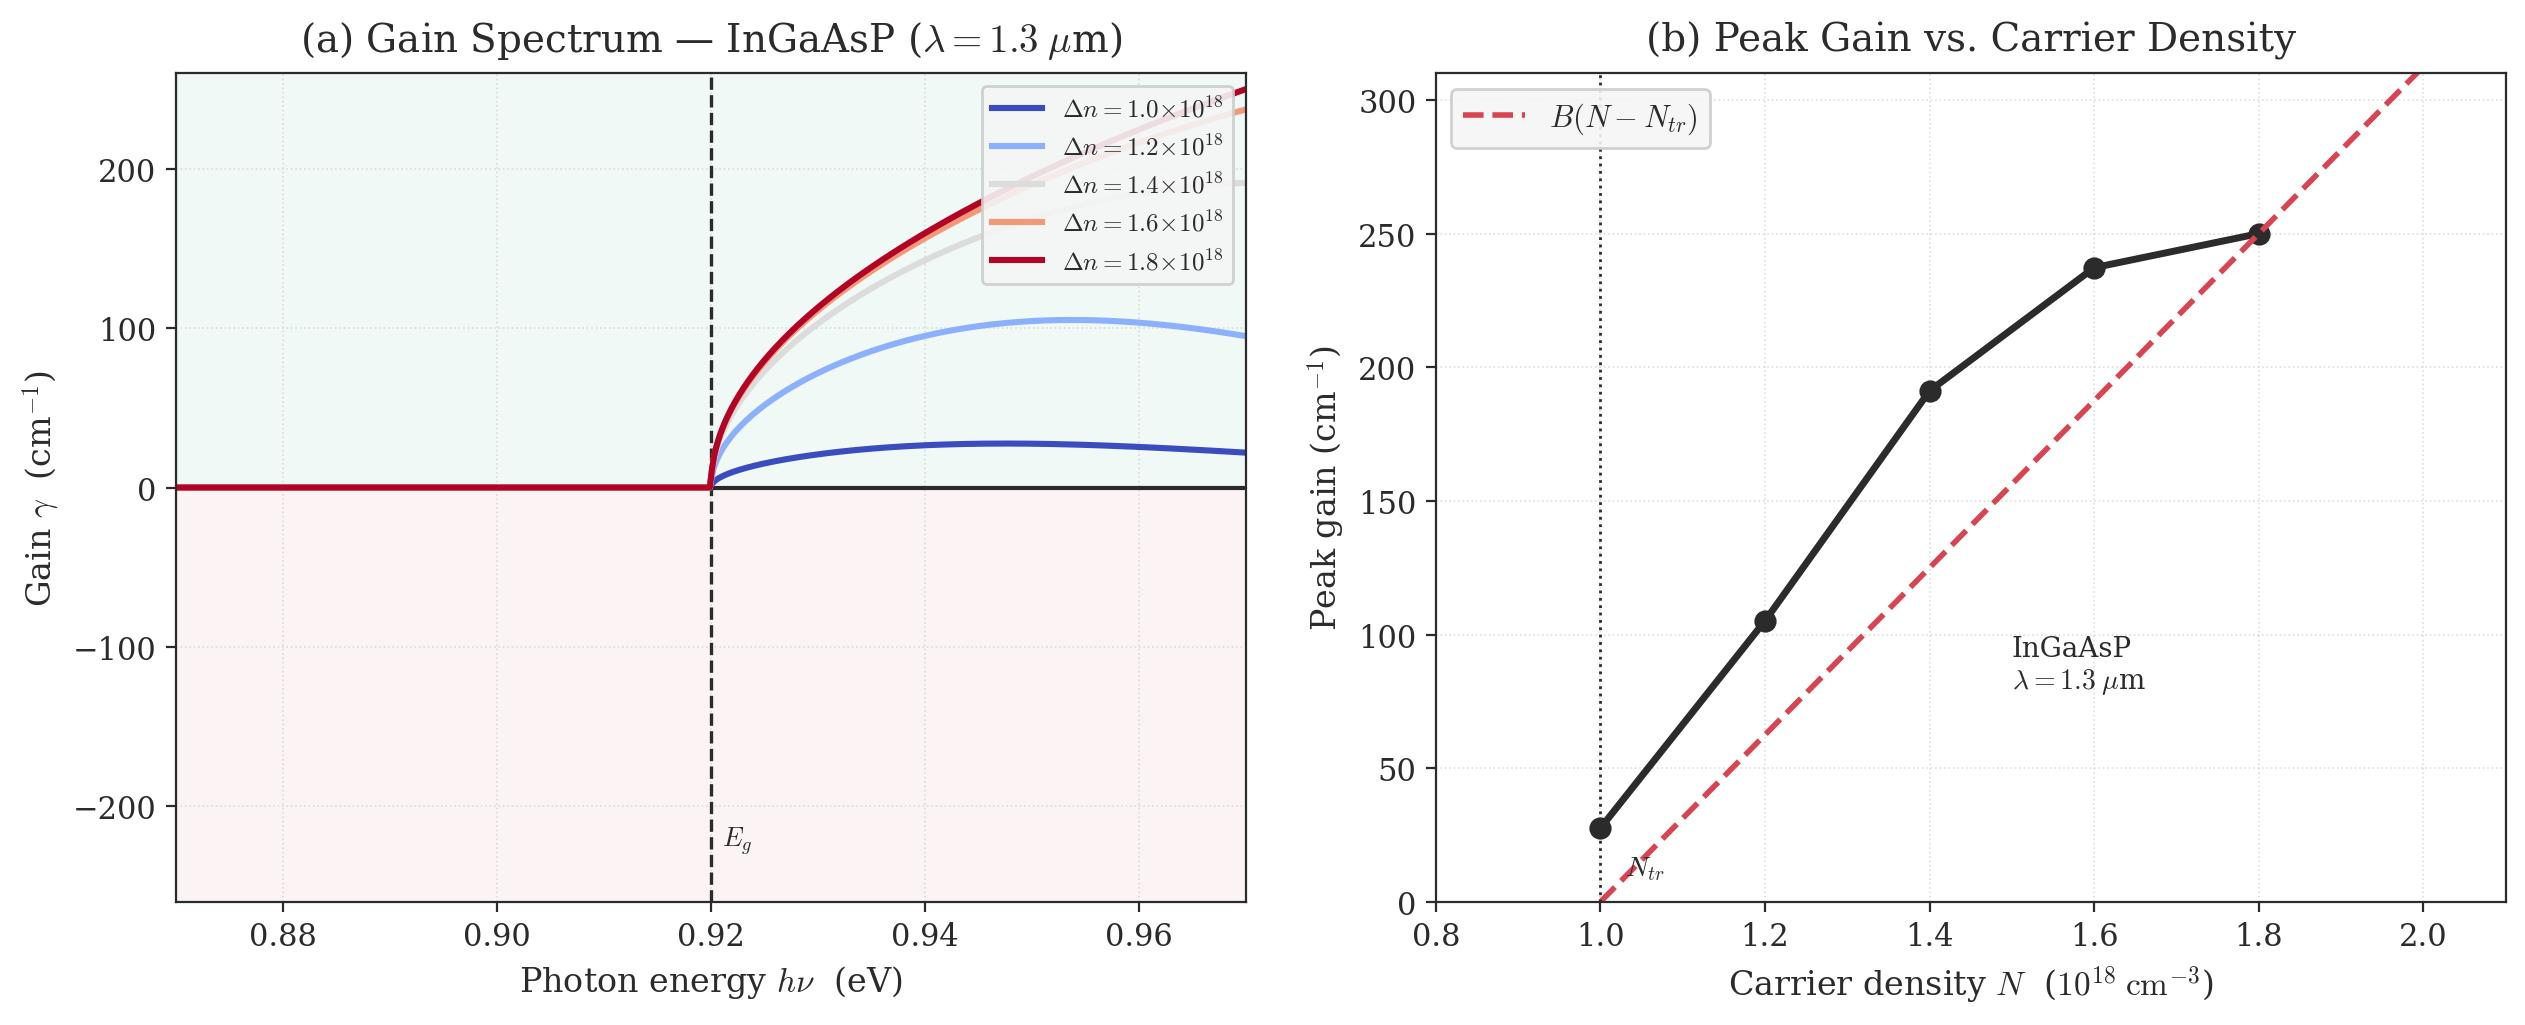
\includegraphics[width=0.75\textwidth]{Figures/Chapter 7/gain_spectrum_and_linear_model.jpg}
    \caption{Linear Gain Approximation: Gain vs. Carrier Density}
    \label{fig:gain_spectrum_and_linear_model}
\end{figure}

% ------------------------------------------------------------------
\section{From Dynamics to Devices}
% ------------------------------------------------------------------

With the carrier rate equation now fully established, we have a complete dynamical framework describing how carriers are injected, how they recombine through competing channels, and how they interact with the photon field. The rate equation $dN/dt = J/(ed) - N/\tau - \Gamma G S$ is the master equation from which all semiconductor device behaviour follows — LED output power, laser threshold, modulation bandwidth, and amplifier gain saturation are all consequences of solving this equation (and its companion photon rate equation) under different operating conditions.

\begin{keyinsight}[The Distinction Between an LED and a Laser Diode]
    Both an LED and a laser diode use the same DH structure, the same material system, and the same current-injection principle. The fundamental difference lies in which term in the rate equation dominates the photon output.

    In an LED, the stimulated emission term $\Gamma G S$ is negligible — either because the photon density is low (no optical feedback) or because the carrier density never reaches the transparency point. All photons are produced by the $N/\tau_r$ spontaneous emission term. The output is incoherent, broad-spectrum, and proportional to current.

    In a laser diode, once the current exceeds the threshold value, stimulated emission dominates completely. The spontaneous term $N/\tau_r$ becomes negligible compared to $\Gamma G S$, and almost every carrier injected above threshold generates a coherent, in-mode photon. The output is coherent, narrow-spectrum, and rises linearly with current above threshold.

    Understanding this distinction — which is fundamentally about whether stimulated emission is negligible or dominant — is the starting point for all that follows.
\end{keyinsight}

The next chapter puts this rate equation to work: we will solve it under steady-state conditions for an LED to calculate its output power, spectral shape, and modulation bandwidth, and then extend the analysis to the semiconductor optical amplifier and the laser diode to derive the threshold condition, the characteristic P–I curve, and the coupled photon-carrier dynamics.
